\section{Design af filter}\label{sec:design_filter}
    Parametre som brugeren skal kunne justere: Centerfrekvensen $\omega_0$,  forstærkning $G$,  filterets godhed $Q$ som bla. beskriver båndbredden på pasbåndet.\\
    Øvrige parametre:
    $G_0$ er reference forstærkning (sættes til 1 for at kunne kaskadekoble flere bånd) og $G_B$ som er forstærkning ved knækfrekvenserne (typisk 3dB over/under fra analog filterteori).s

    \subsection{Analog filter}

	Som filter til equalizeren anvendes high-shelf, low-shelf og  peak/notch.
    Der bliver kun anvendt 2. ordens filtre, da der ikke er brug for højere orden inde for audio. 

     \subsection{Peak/notch filter}

    Et peak/notch filter i en parametrisk equalizer består af et båndpas-, $H_{BP}$, og et båndstopfilter, $H_{BS}$. 
    Et analogt båndpasfilter kan beskrives med ligning \ref{eq:iir_bandpas} 
    hvor $\alpha$ er en konstant der er afhængig af frekvensspecifikationer, $\Omega_0$ er centerfrekvensen.\\
    I ligning \ref{eq:iir_bandstop} er en overføringsfunktion for et båndstopfilter.
    I ligning \ref{eq:iir_peaknotch} summeres båndstop- og båndpasfilteret for at kunne forstærke eller dæmpe signalet omkring center frekvensen.    
     \begin{align}
     H_{NOTCH}(s) &= \dfrac{s^2 + \Omega_0^2}{s^2 + \alpha s + \Omega_0^2}
     \label{eq:iir_bandpas} \\
     H_{PEAK} (s) &= \dfrac{\alpha s}{s^2 + \alpha s + \Omega_0^2}  
     \label{eq:iir_bandstop} \\
     H_a (s) &= G_0 H_{NOTCH} (s) + G H_{PEAK} (s) = \dfrac{G_0 (s^2 + \Omega_0^2) + G \alpha s}{s^2 + \alpha s + \Omega_0^2}
     \label{eq:iir_peaknotch}
    \end{align}
    Filterets gain kan bestemmes ud fra ligning \ref{eq:iir_gain}.
    \begin{align}
        G_B = \dfrac{G_0^2 + G^2}{2} \label{eq:iir_gain}
    \end{align}

    Ved at sætte $s = j \Omega$ i ligning \ref{eq:iir_bandpas} og \ref{eq:iir_bandstop}, og sætte $\big| H(j\omega)\big|^2 = G_B^2$, hvor $G_B^2$ er den ønskede forstærkning ved den ønskede centerfrekvens $\Omega_0$, kan parameteren $\alpha$ findes for de givne specifikationer.
   I kilde \cite{Orfanidis1996} udledes at udtryk (ud fra ligning \ref{eq:h_a_gb}) for $\alpha$ hvori $\beta$ defines som i ligning \ref{eq:beta_calc}. 
   % \begin{align}
   %  |H_{a}(j \Omega)| = \dfrac{G_0 (\Omega_0^2- \Omega^2)+ j G \alpha \Omega}{-\Omega^2 + j \alpha \Omega + \Omega_0^2}   
  %  \end{align}

    \begin{align}
        |H_{a}|^2 &= G_B^2 =  \dfrac{(\Omega_0^2- \Omega^2)^2 + G^2 \alpha^2 \Omega^2}{(\Omega_0^2-\Omega^2)^2 +\alpha^2 \Omega^2}  % \iff \Omega^4 - \left(2 \Omega_0^2 + \dfrac{G^2- G_B^2}{G_B^2- G_0^2} \alpha^2 \right) \Omega^2 + \Omega_0^4 =0
        \label{eq:h_a_gb}\\
       \Delta \Omega^2 &= (\Omega_2 - \Omega_1 )^2 = \dfrac{G^2 - G_B^2}{G_B^2 - G_0^2}  \alpha^2 \rightarrow \Delta \Omega = \sqrt{\dfrac{G^2 - G_B^2}{G_B^2 - G_0^2}} \alpha \iff \alpha = \sqrt{\dfrac{G_B^2-G_0^2}{G^2 - G_B^2 }} \Delta \Omega
       \label{eq:beta_calc}
    \end{align}


    \begin{align}
    \beta \equiv \dfrac{\alpha}{(1 + \Omega_0^2)}    = \sqrt{\dfrac{G_B^2-G_0^2}{G^2 - G_B^2 }} \tan \left( \dfrac{\Delta \omega}{2} \right) \label{eq:beta}
    \end{align}


    \subsection{Bilinear Transformation}
    Ud fra overføringsfunktionen $H_a(s)$ udskiftes $s$ med $z$ for at få $H(z)$ som ses i \ref{eq:iir_replace_s}.
    \begin{align}
    s =   \dfrac{z^{-1} - 1}{z^{-1} + 1} \label{eq:iir_replace_s}
    \end{align}
	$H_a(s)$ transformeres med ligning \ref{eq:iir_replace_s} om til $H(z)$ i ligning \ref{eq:iir_omskriv_til_z}.
    \begin{equation}
    H_a(z) = H_a(S)\bigg|_{S = \frac{z^{-1} -1 }{z^{-1} + 1}} \label{eq:iir_omskriv_til_z}
    \end{equation}
    Fordelen med denne transformation er at ordenen på $H(z)$ er denne samme som $H(z)$. Hvis $H_a(s)$ er stabil og kausal, så er $H(z)$ også.
    
    I ligning \ref{eq:iir_peak_tfz} ses overføringsfunktionen for et peak notch filter.
   \begin{align}
    H(z) = H_a(s)\bigg|_{s = \frac{z^{-1} -1 }{z^{-1} + 1}} = 
    \dfrac{\left(\dfrac{G_0 + G \beta}{1 + \beta} \right)- 2 \left(\dfrac{G_0 cos( \omega_0)}{1 +\beta} \right)z^{-1} + \left(\dfrac{ G_0 - G \beta}{1 + \beta }\right) z^{-2}}{1 - 2 \left(\dfrac{cos(\omega_0)}{1 + \beta}\right)z^{-1} + \left( \dfrac{1 - \beta}{1 + \beta} \right) z^{-2}}
    \label{eq:iir_peak_tfz}
   \end{align}

   Hvor parametrene er $\Delta \omega$, $G$, $f_0$. Heraf beregnes $w_0$ udfra ligning \ref{eq:freq_warp_w0}, $\Delta \omega$ udfra ligning \ref{eq:freq_warp_BW}, $\beta$ fra ligning \ref{eq:beta}, $G_B$ beregnes fra ligning \ref{eq:iir_gain}.
   På figur \ref{fig:iir_peak} betragtes indflydelsen fra båndbredden $\Delta \omega$, når den varierer.

 \begin{figure}
    \centering
         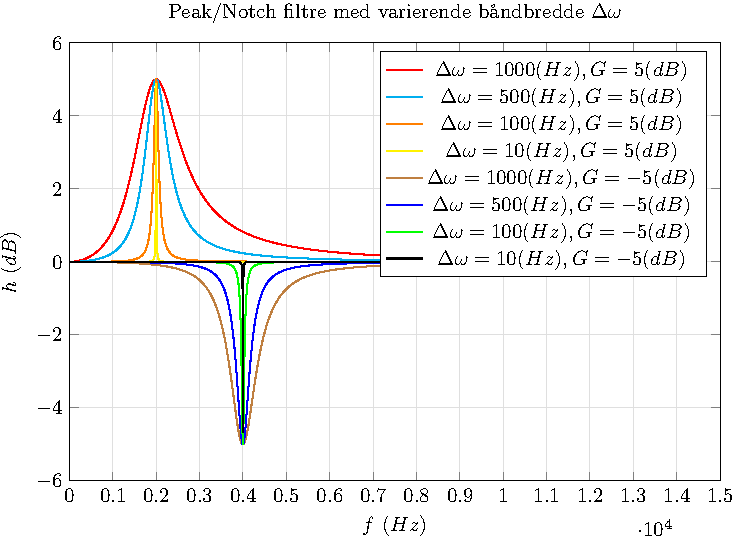
\includegraphics{figure/iir_peak-crop.pdf}
        \caption{Peak/notch filtre med centerfrekvens $f_0 = 2kHz$ og $f_0 = 4kHz$, varierende $\Delta \omega$ og gain $G=5dB$}
        \label{fig:iir_peak}   
    \end{figure} 
\FloatBlock

     \subsection{Low-shelf filter}

   %  \begin{align}
    %     H_{LS}(z) = \dfrac{\sqrt{G} \left( \sqrt{G} \Omega^2 + \sqrt{2} \Omega G^{\frac{1}{4}} + 1 \right) +2 \sqrt{G} \left( \sqrt{G} \Omega^2 - 1\right) z^{-1} + \sqrt{G} \left(\sqrt{G} \Omega^2- \sqrt{2} \Omega G^{\frac{1}{4}} + 1 \right) z^{-2}}{\sqrt{G} + \sqrt{2} \Omega G^{\frac{1}{4}} + \Omega^2 + 2 \left( \Omega^2 - \sqrt{G} \right) z^{-1} + \left(\sqrt{G} -\sqrt{2} G^{\frac{1}{4}} + \Omega^2 \right) z^{-2}}
    % \end{align}
	
	For at komme fra overføringsfunktionen for peak / notch filteret (\ref{eq:iir_peak_tfz}) til et low shelf filter, sættes $\omega_0 = 0$, for at få de led med $\omega_0$ til at udgå fra ligningen. 
	Forstærkningen ved knækfrekvensen $G_C$ defineres ligeledes $G_B$ i peak/notch filteret.
    Heraf kommer udtrykket for $\beta$, som ses i ligning \ref{eq_iir_beta}.
    \begin{align}
        H_a (s) &= \dfrac{G_0 s + G \beta}{s + \beta} \nonumber \\
        |H_a (\Omega)|^2 &= \dfrac{G_0^2 \Omega^2 + G^2 \beta^2}{\Omega^2 + \beta^2} = G_C^2 \nonumber \\
        \beta &= \sqrt{\dfrac{G_C^2 - G_0^2}{G^2 - G_C^2}} \tan \left( \dfrac{\omega_c}{2} \right) \label{eq_iir_beta}
    \end{align}
	Herefter indsættes $\beta$ i overføringsfunktionen for low shelf filteret og opskrives i ligning \ref{iir_low_shelf}.
     \begin{align}
      H_{LS}(z) =   \dfrac{\left(\dfrac{G_0 + G \beta}{1 + \beta} \right)+ \left(\dfrac{ G_0 - G \beta}{1 + \beta }\right) z^{-1}}{1 + \left( \dfrac{1 - \beta}{1 + \beta} \right) z^{-1}} \label{iir_low_shelf}
     \end{align}
	Lowshelf filteret er plottet i figur \ref{fig:iir_low_shelf} med variende gain, $G$.
%    \begin{figure}[h]
%    \centering
%        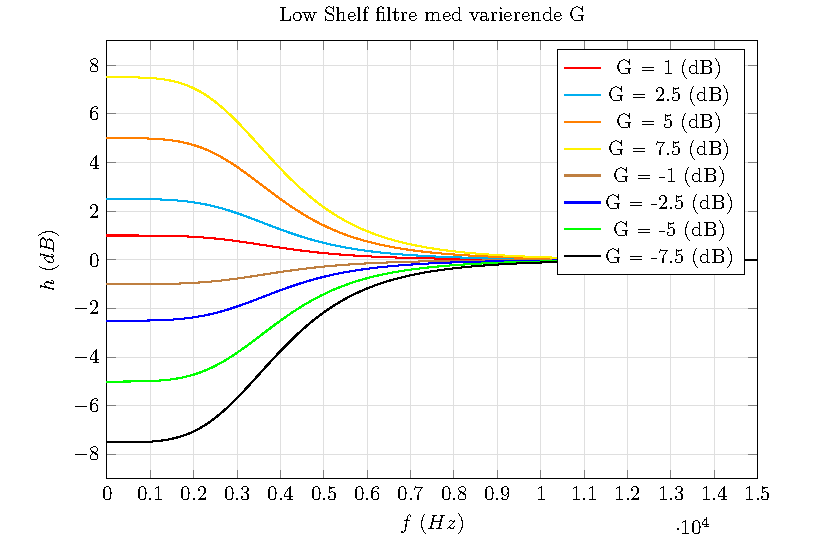
\includegraphics{figure/iir_ls.pdf}
%        \caption{Low shelf filter med knækfrekvens $f_c = 4kHz$, varierende gain $G$ i intervallet: $[-7.5 ; 7.5]$} \label{fig:iir_low_shelf_test}
%    \end{figure}
%	\FloatBlock 
   
   
     \subsection{High-shelf filter}
	I et high-shelf filter tages der ligesom i low-helf filteret udgangspunkt i ligning \ref{eq:iir_peak_tfz}. Modsat low-shelf filteret sættes $\omega_0 = \pi$.
	Overføringsfunktionen for high-shelf filterets opskrives i ligning \ref{iir_hs_tf}.
     \begin{align}
        H_a (s) = \dfrac{G_0 + G \beta s}{1 + \beta s} \label{iir_hs_tf}
     \end{align}
	I ligning \ref{iir_hs_tf_size} findes størrelsen af amplituderne.
     \begin{align}
         |H_a(\Omega)|^2 = \dfrac{G_0^2 + G^2 \beta^2 \Omega^2}{1 + \beta^2 \Omega^2} = G_C^2 \label{iir_hs_tf_size}
     \end{align}
     For at simplificere udtrykket, laves en omskrivning i ligning \ref{iir_beta_helper}. Her indføres knækfrekvensen $\omega_c = \pi - w_0$ og $\omega_0 = \pi$ hvilket vil sætte centerfrekvensen i $f = \infty$, båndbredden bliver heraf knækfrekvensen til high-shelf filteret.
    \begin{align}
        \beta = \sqrt{\dfrac{G_C^2 - G_0^2}{G^2 - G_C^2}} \tan \left( \dfrac{\pi - \omega_c}{2} \right) \label{iir_beta_helper}
    \end{align}

    %  \begin{align}
     %    H_{HS} = \dfrac{\sqrt{G} \left(  \sqrt{G} + \sqrt{2} \Omega G^{\frac{1}{4}}+ \Omega^2 \right) -2 \sqrt{G} \left( \sqrt{G} - \Omega^2 \right) z^{-1} + \sqrt{G} \left(\sqrt{G} - \sqrt{2} \Omega G^{\frac{1}{4}} + 1 \right) z^{-2} }{arg}
     %\end{align}


     For at beregne $\beta$ anvendes ligning (\ref{eq:beta}), hvorefter $cos(\omega_0) = cos(\pi) = -1$. Dette giver overføringsfuntionen for high-shelf filteret som ses i ligning \ref{iir_hs_tf_z}, og er en forkortet udgave peak/notch filtrenes overføringsfuntion. Et plot af high-shelf filteret ses i figur \ref{fig:iir_high_shelf}.
     \begin{align}
     H_{HS}(z) =     \dfrac{\left(\dfrac{G_0 + G \beta}{1 + \beta} \right) + \left(\dfrac{ G_0 - G \beta}{1 + \beta }\right) z^{-1}}{1  + \left( \dfrac{1 - \beta}{1 + \beta} \right) z^{-1}} \label{iir_hs_tf_z}
     \end{align}
%
%
% \begin{figure}[h]
%      \centering
%        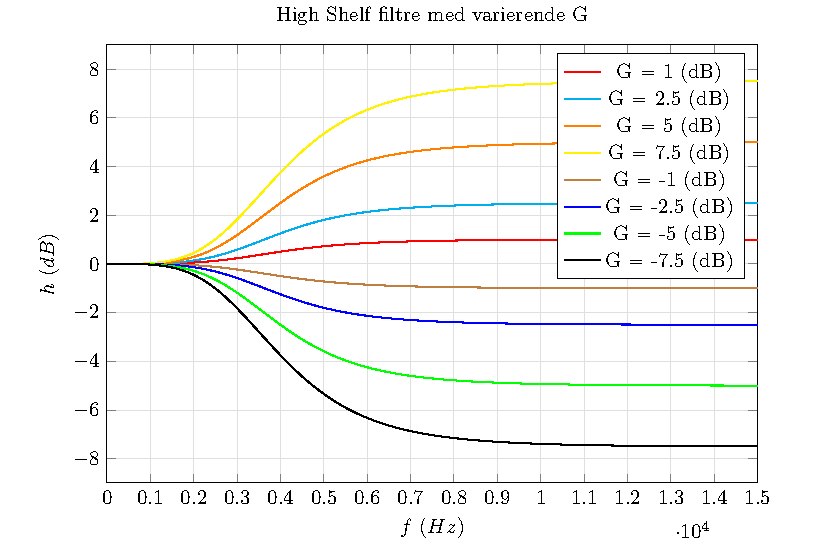
\includegraphics[]{figure/iir_hs.pdf}
%        \caption{High shelf filter med knækfrekvens $f_c = 4kHz$, varierende gain $G$ i intervallet: $[-7.5 ; 7.5]$} \label{fig:iir_high_shelf}
%   \end{figure}  


\begin{figure}[h]
	\centering
	\subbottom[]{%
		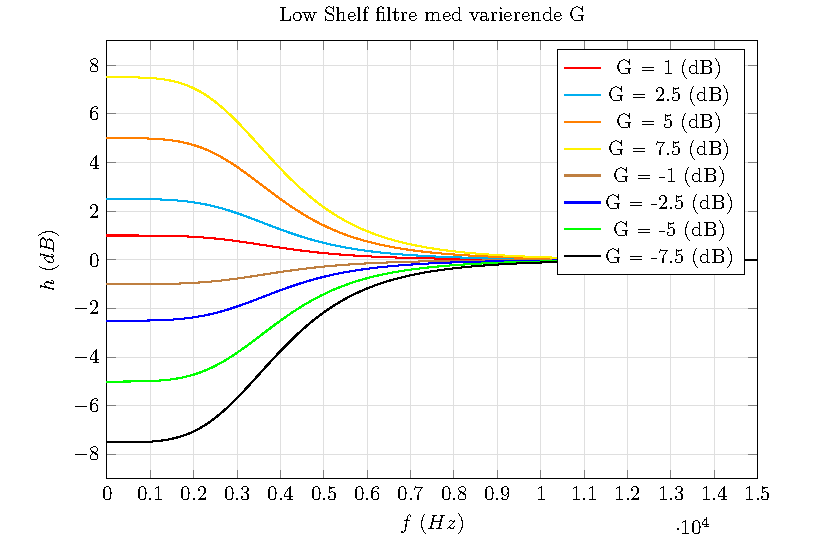
\includegraphics[width=7.35cm]{figure/iir_ls.pdf}
		\label{fig:iir_low_shelf}}
	\subbottom[]{%
		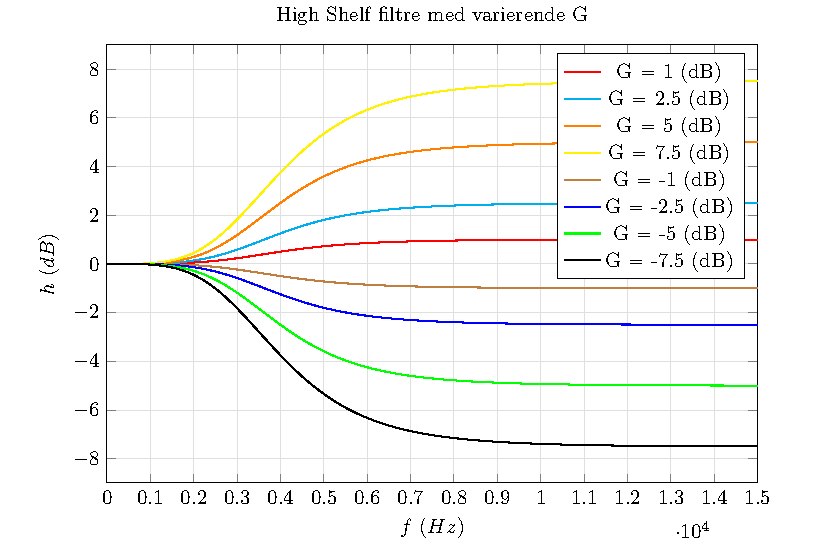
\includegraphics[width=7.35cm]{figure/iir_hs.pdf}
		\label{fig:iir_high_shelf}}
	\caption{\ref{fig:iir_low_shelf}: Low shelf filter. \hspace{4cm} \ref{fig:iir_high_shelf}: High shelf filter. \newline Begge filtre har en knækfrekvensen $f_c = 4kHz$ og et gain $G$ i intervallet: $[-7.5 ; 7.5]$}
\end{figure}
\FloatBlock

\subsection{Fejl ved Bilinear Transformation}


\section{Realisering af filter}

Differensligningen er beskrevet med ligning \ref{eq:diffrens}, dette kan illustreres vha. et blok diagram figur (\ref{fig:real_diag}). 

    \begin{align}
    y(n) = \sum\limits_{i=0}^{M} b_i x(n-i) - \sum\limits_{i=1}^N a_i y(n-i)
    \label{eq:diffrens}
    \end{align}


   \begin{figure}[h]
        \centering
        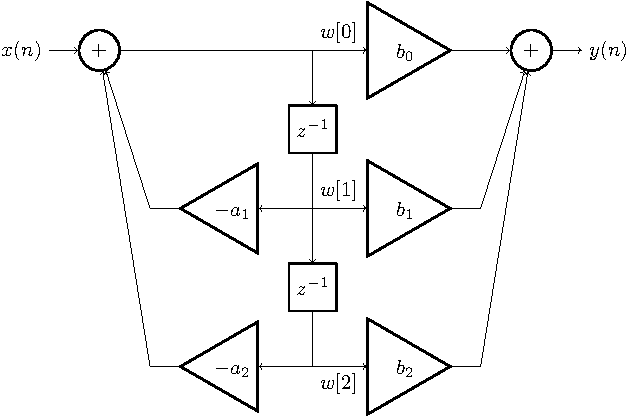
\includegraphics[scale = 0.8]{figure/iir_sos-crop.pdf}
        \caption{Realiserings diagram af 2. ordens iir filter. }    
        \label{fig:real_diag}
    \end{figure}

   Ud fra blokdiagrammet \ref{fig:real_diag} kan iir-filteret beskrives med ligning \ref{eq_iir_diff_real} 
   hvor $b_i$ er filterets tæller koefficienter, $a_i$ er filterets nævner koefficienter og $w$ indeholder 
   værdier fra de tidligere filtrede samples. Efter $y[n]$ er beregnet skubbes værdierne i $w$ variablen  
 således at de passer til det nye filtrede samples. 
    \begin{align}
        w[0] &=x[n] - w[1] \cdot a_1 - w[2] \cdot a_2 \\
        y[n] &= w[0] \cdot b_0 + w[1] \cdot b_1 + w[2] \cdot b_2
        \label{eq:iir_diff_real}
        \\
        w[2] &= w[1] \\
        w[1] &= w[0]
    \end{align}

    Da filteret er afhængig af de tidligere værdier skal det filtrere et par samples således at all $w$ variablene 
    har fået tildelt sig en værdi.
Når de forskellige 2. ordensfiltre skal kaskadekobles. Hvis $x_{1}[n]$ repræsenterer det sample der filtres af det 1. bånd så vil $x_{2}[n] = y_{1}[n]$.
    Dvs. at ligning \label{eq:iir_diff_real} beregnes per bånd af equalizeren hvor det samlet antal bånd betegnes $K$.\\
\subsection{Repræsentering af koefficienter}

    Koefficienterne haves i $K \times 3$ matricer,
    $A_K$ er nævner polynomie matricen, $B_K$ er tæller polynomie matricen
   og $W_K$ er state-variablene hvilket kan ses i ligning \ref{eq:matrix_states}.  

   \begin{align}
   A_{Kj} = \left[\begin{matrix}
   1 			& a_{01} 	& a_{02} \\
   1 			& a_{11} 	& a_{12} \\
   1 			& a_{21} 	& a_{22} \\
   \vdots 		& \vdots 	&  \vdots \\
   1 			& a_{K1} 	& a_{K2} \\
   \end{matrix}
   \right], \quad
      B_{Kj} = \left[\begin{matrix}
   b_{00}		& b_{01} 	& b_{02} \\
   b_{10}		& b_{11} 	& b_{12} \\
   b_{20}		& b_{21} 	& b_{22} \\
   \vdots 		& \vdots 	&  \vdots \\
   b_{K0}		& b_{K1} 	& b_{K2} \\
   \end{matrix}
   \right], \quad
      w_{Kj} = \left[\begin{matrix}
   w_{00}		& w_{01} 	& w_{02} \\
   w_{10}		& w_{11} 	& w_{12} \\
   w_{20}		& w_{21} 	& w_{22} \\
   \vdots 		& \vdots 	&  \vdots \\
   w_{K0}		& w_{K1} 	& w_{K2} \\
   \end{matrix}
   \right]
   \label{eq:matrix_states}
   \end{align}

   Koefficienterne haves i floating point format. For at effektivisere beregningerne aktiveres floating point 
   enheden. 


\section{Frekvensrepons af Amplituden}

Ved at bruges ligning (\ref{eq:z_to_amp}) hvori amplituden findes fra (\ref{eq:complex_to_amp}).

\begin{align}
    z= e^{j \Omega} = \cos{\Omega} + j \sin{\Omega}  
    \label{eq:z_to_amp}\\
    |H(\Omega)| = \sqrt{ \Re{(H)}^2  + \Im{(H) }^2 }
    \label{eq:complex_to_amp}
\end{align}

Da de individuelle filtre er af 2. orden kan amplituden regnes:

\begin{align}
    H(\omega) &= \prod\limits_{i=0}^{K-1} \dfrac{b_{i0} + b_{i1} z^{-1} + b_{i2} z^{-2}}{a_{i0} + a_{i1} z^{-1} + a_{i2} z^{-2}} \nonumber
    \\ &= \prod\limits_{i=0}^{K-1} \dfrac{b_{i0} + b_{i1} \left( \cos{\Omega} + j \sin{\Omega} \right)+b_{i2} \left( \cos{2\Omega} + j \sin{2\Omega} \right)}{a_{i0} + a_{i1} \left( \cos{\Omega} + j \sin{\Omega} \right)+a_{i2} \left( \cos{2\Omega} + j \sin{2\Omega} \right)}
\end{align}
Hvis $H(\Omega)$ deles op i hhv. $N(\Omega)$ tæller, $D(\Omega)$ nævner kan amplituden for en 
given frekvens $\Omega$ findes ved ligning (\ref{eq:amp_calc}).

\begin{align}
    |H(\Omega)| &= \sqrt{ \dfrac{\Re{(N(\Omega))}^2 + \Im{(N(\Omega))}^2 }{\Re{(D(\Omega))}^2 + \Im{(D(\Omega))}^2 }} \nonumber	\\ 
     &= \prod\limits_{i=0}^{K-1} \dfrac{ \sqrt{\left( b_{i0} + b_{i1} \cos{\Omega} + b_{i2} \cos{2 \Omega} \right)^2 +  \left( b_{i1} \sin{\Omega} + b_{i2} \sin{2 \Omega} \right)^2 } }{ \sqrt{\left( a_{i0} + a_{i1} \cos{\Omega} + a_{i2} \cos{2 \Omega} \right)^2 + \left( a_{i1} \sin{\Omega} + a_{i2} \sin{2 \Omega} \right)^2} }
    \label{eq:amp_calc}
\end{align}

Denne ligning er den samlet beren

\section{Delkonklusion}

\note{
	Test af CPU og hvordan det er at implementere
}